\setcounter{subsection}{0}
\section{DISEÑO DE LA SOLUCIÓN}

El diseño se documentó en el SDD (IEEE 1016, ISO/IEC/IEEE 42010) con el modelo C4 y UML. Esta sección resume la arquitectura, los datos, los algoritmos principales y las decisiones tecnológicas.

\subsection{Objetivos y prioridades de diseño}

Las decisiones se tomaron según cinco prioridades, en este orden: (1) \textbf{reproducibilidad}: la misma entrada debe producir la misma salida; (2) \textbf{mantenibilidad}: un estudiante nuevo debe poder entender cada etapa; (3) \textbf{respuesta fluida con un simulador lento}, ya que una corrida completa tarda unos 12 minutos; (4) \textbf{verosimilitud sin sobreprometer}: declarar lo que no se modela; y (5) \textbf{operación local y simple}, sin base de datos ni nube.

\subsection{Arquitectura}

El sistema es una aplicación cliente–servidor local, un monolito modular. La figura~\ref{fig:contenedores} muestra los contenedores (nivel 2 del modelo C4): el navegador carga el visor (React, kepler.gl, three.js); el servidor de desarrollo de Vite reenvía \texttt{/api/*} (HTTP y WebSocket) a una API FastAPI, que orquesta las herramientas de SUMO como subprocesos y lee y escribe en el sistema de archivos.

\begin{figure}[H]
\centering
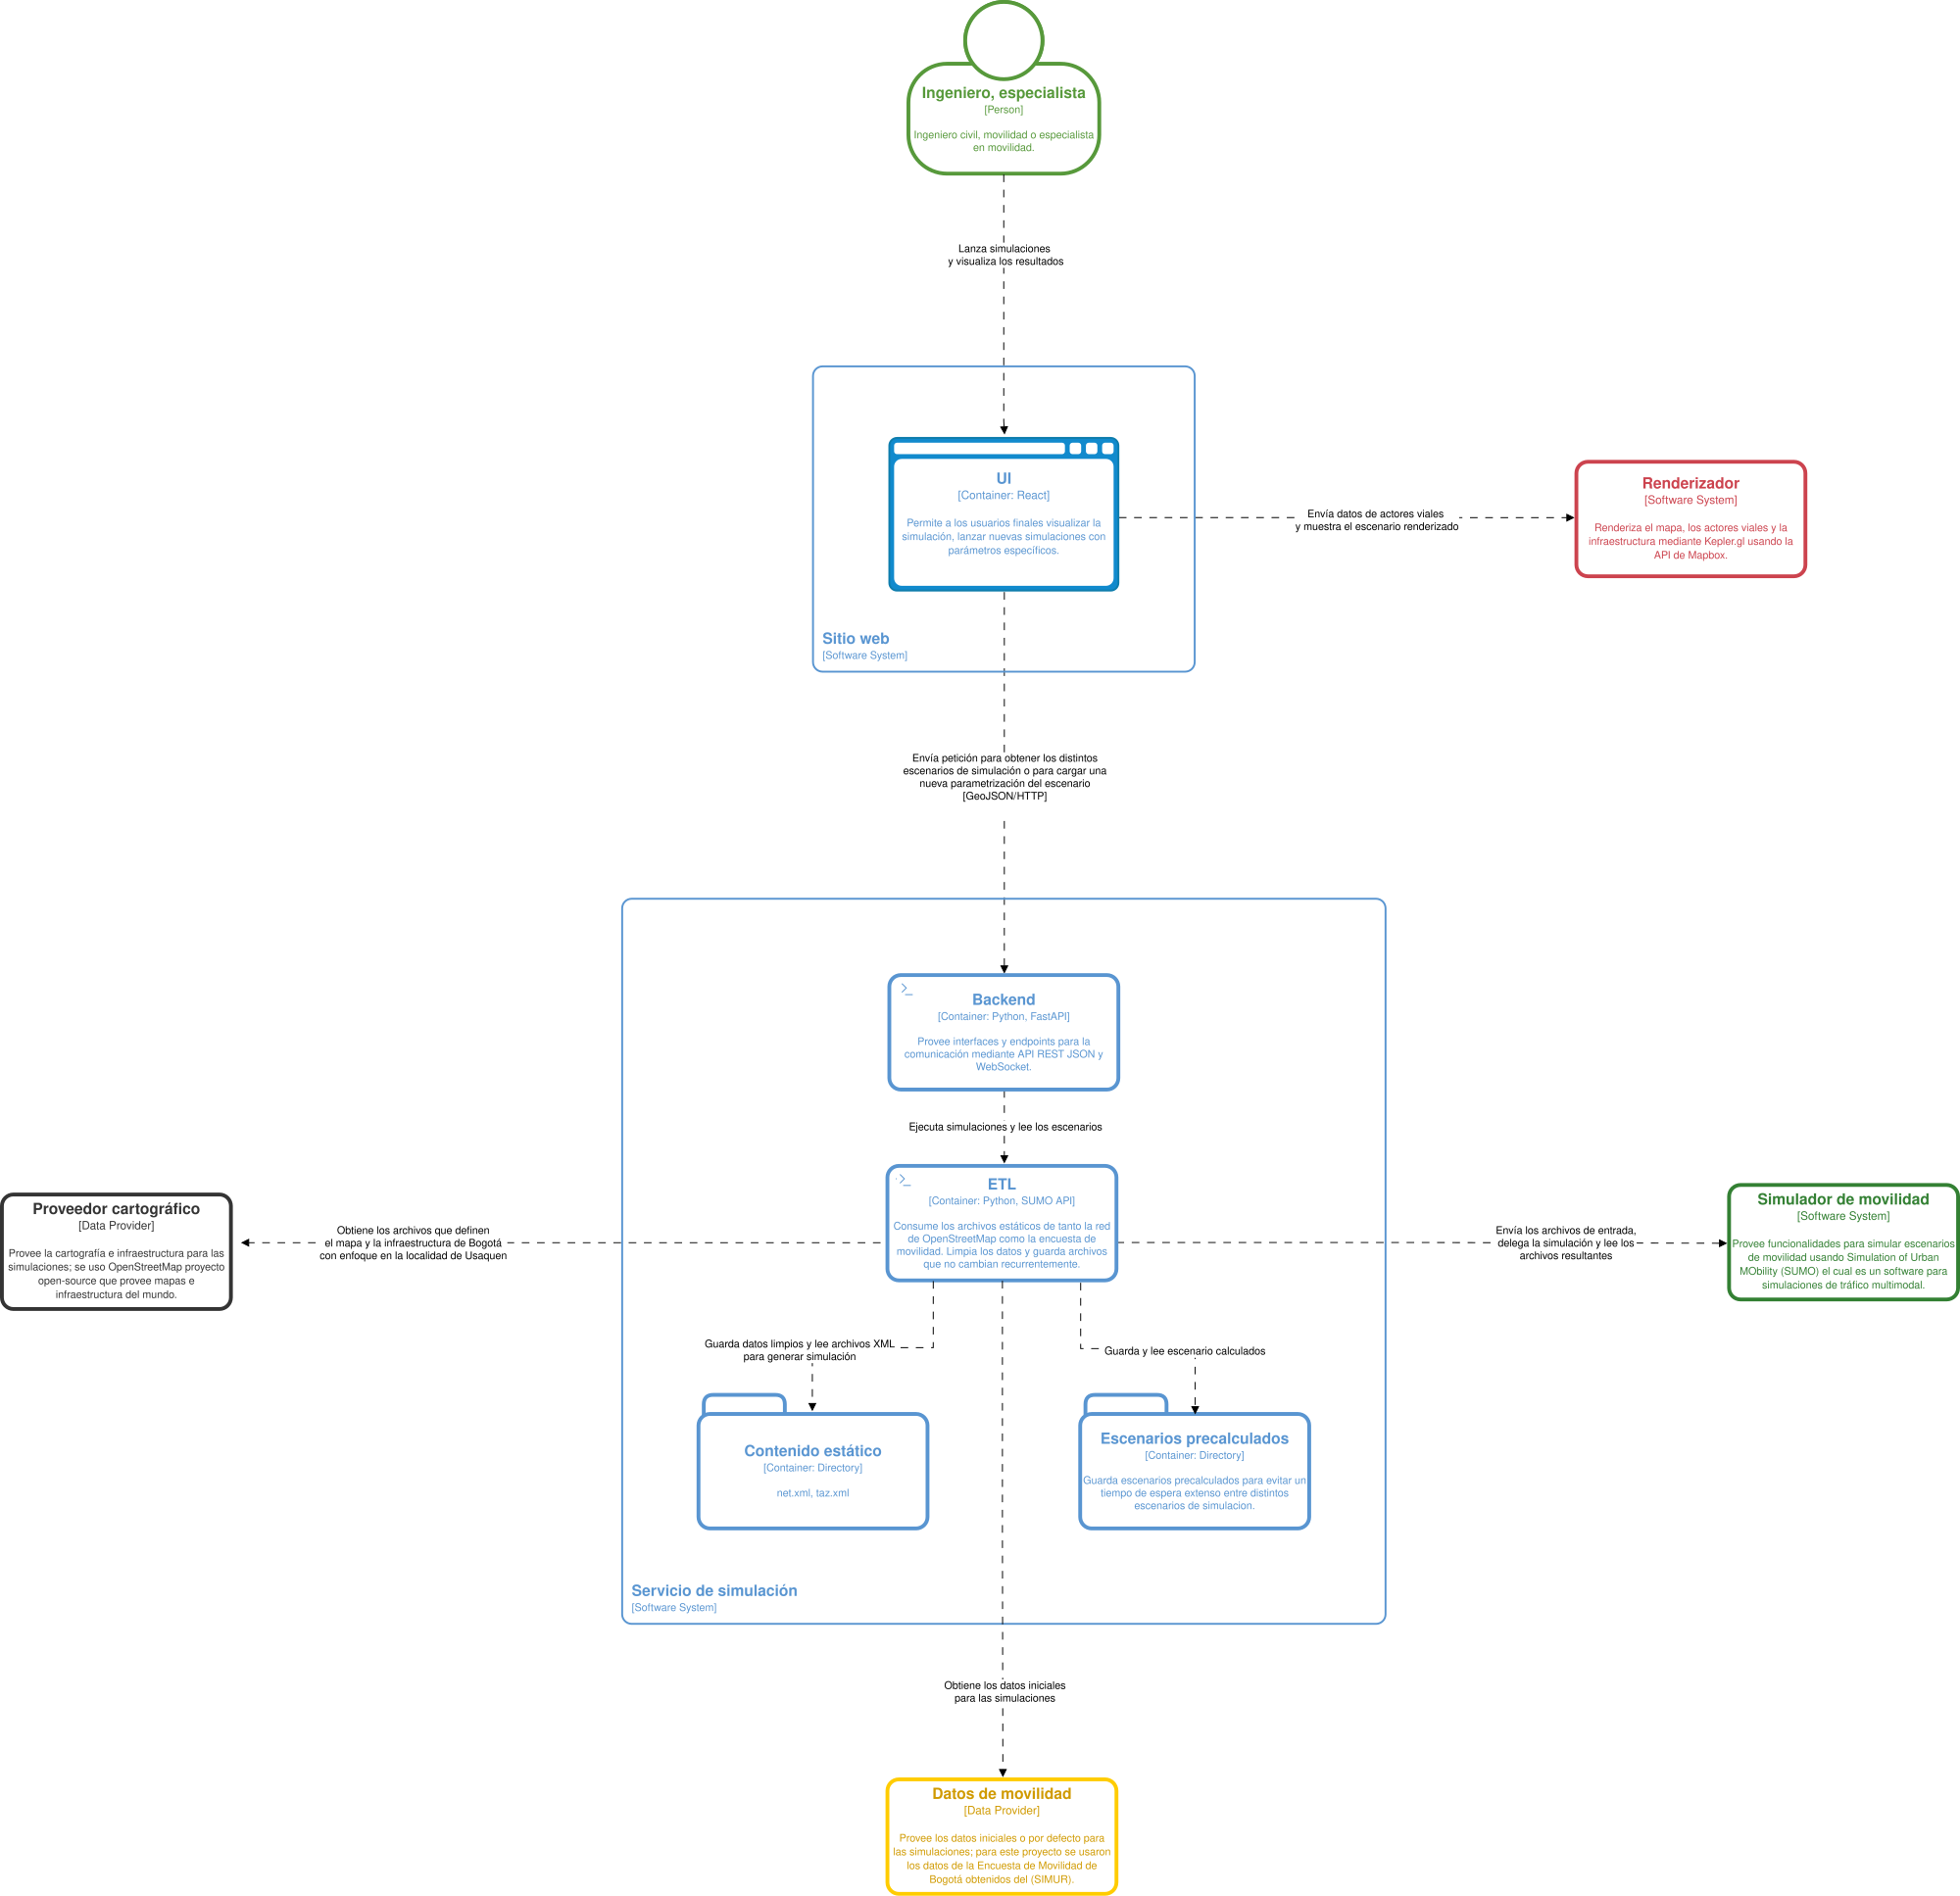
\includegraphics[width=0.95\textwidth]{c4-contenedores.png}
\caption{Diagrama de contenedores del sistema (modelo C4, nivel 2).}
\label{fig:contenedores}
\end{figure}

La arquitectura tiene cuatro capas (tabla~\ref{tab:capas}). Dentro del servicio conviven tres estilos: una \textit{tubería de etapas} para el ETL (cada etapa lee los archivos de la anterior y escribe los suyos); \textit{trabajos asíncronos con un solo trabajador} para las corridas largas (la API responde \texttt{202 Accepted} y el cliente consulta el estado cada 2~s); y un \textit{flujo en tiempo real por WebSocket} para el simulador 3D, donde dos instancias de SUMO avanzan en lockstep y el servidor emite un cuadro por paso.

\begin{table}[ht]
\renewcommand{\arraystretch}{1.15}
\centering
\small
\begin{tabular}{|p{3cm}|p{11cm}|}
\hline
\textbf{Capa} & \textbf{Responsabilidad} \\ \hline
Presentación & Visor: mapa kepler.gl, paneles de demanda, ficha de intersección, semaforización y simulador 3D (carga diferida). \\ \hline
Interfaz (API) & Validación de peticiones con Pydantic, códigos HTTP y WebSocket; sin lógica pesada. \\ \hline
Orquestación & \texttt{GestorCorridas} (corridas en segundo plano) y \texttt{GestorComparaciones} (comparaciones 3D con TraCI). \\ \hline
Dominio y datos & Paquete \texttt{etl}: demanda, ruteo, simulación, exportación, intersecciones, priorización, escena 3D y telemetría. \\ \hline
\end{tabular}
\caption{Capas de la arquitectura.}
\label{tab:capas}
\end{table}

\textbf{Modularidad.} Todos los módulos de \texttt{etl/sumo/} siguen el mismo patrón: un \texttt{*Config} inmutable (con \texttt{to\_args()} si invoca una herramienta de SUMO), un \texttt{*Result} y un \texttt{*Stats} mutable que acumula contadores (por ejemplo, filas inválidas y viajes generados). Los envoltorios de subprocesos ubican el binario con \texttt{shutil.which} y lanzan una excepción propia; los procesos largos aceptan un \textit{callback} de avance y un evento de cancelación. \texttt{configuration.py} es la única fuente de rutas y constantes.

\subsection{Diseño de datos}

El sistema no usa motor de base de datos: los datos son archivos (TSV, XML de SUMO, JSON y GeoJSON) organizados por escenario (\texttt{scenarios/<nombre>/}) y por corrida (\texttt{runs/<id>/}), y las estructuras en memoria son \texttt{dataclass}. La entrada de todo el sistema es el TSV de viajes internos de Usaquén (2.580 filas), filtrado en los cuadernos de exploración. La tabla~\ref{tab:tsv} describe sus campos relevantes.

\begin{table}[ht]
\renewcommand{\arraystretch}{1.15}
\centering
\small
\begin{tabular}{|p{3.6cm}|p{10.4cm}|}
\hline
\textbf{Campo} & \textbf{Uso} \\ \hline
\texttt{zat\_ori}, \texttt{zat\_des} & Zonas de origen y destino; se mapean a TAZ. La fila es inválida si falta alguna. \\ \hline
\texttt{hora\_ini\_seg} & Hora de salida en segundos desde las 00:00; solo se aceptan viajes entre las 7:00 y las 10:00. \\ \hline
\texttt{duracion\_min} & Duración reportada; define el rango de duración para los presets. \\ \hline
\texttt{modo\_principal\_agrupado} & Etiqueta cruda (11 valores) que se convierte en uno de 10 modos de transporte. \\ \hline
\texttt{fexp\_vj} & Factor de expansión: el viaje se replica $\mathrm{round}(f_{exp})$ veces, con un tope de 50. \\ \hline
\end{tabular}
\caption{Campos del TSV de viajes y su uso.}
\label{tab:tsv}
\end{table}

Las filas inválidas, fuera de ventana o con modo desconocido no se descartan en silencio: se cuentan en un objeto de estadísticas y se reportan. El estado de cada corrida (\texttt{estado.json}) guarda su identificador, estado, etapa, avance, parámetros, resultado y errores; así el historial se reconstruye tras reiniciar el servicio. Las simulaciones precalculadas se guardan con un \texttt{meta.json} que incluye una huella SHA-256 de los insumos para detectar si quedaron obsoletas.

\subsection{Algoritmos principales}

\textbf{Generación de demanda parametrizada.} Un preset (\textit{encuesta}, \textit{más vehículos}, \textit{más peatones}, \textit{día sin carro}) es un conjunto de reglas de transferencia modal que redistribuyen los viajes usando $P(\text{modo}\mid\text{rango de duración})$, calculada de la encuesta completa del día ponderada por \texttt{fexp}. Los presets conservan el total de viajes, y un viaje que cambia de modo mantiene su origen, destino y hora de salida. Los conteos del usuario se reparten entre los viajes de ese modo con el método del mayor resto, de modo que el reparto es determinista. Con el preset \textit{encuesta} y sus conteos por defecto el resultado reproduce exactamente la expansión simple de la encuesta (hay pruebas que lo verifican).

\textbf{Ruteo y simulación.} Los viajes se escriben ordenados por hora de salida. Esto es necesario porque SUMO descarta (sin reordenar) las entidades cuya salida es menor que la máxima ya cargada; sin ordenar se perdían unos 23.000 de los 24.600 viajes. \texttt{duarouter} calcula las rutas con \texttt{--ignore-errors --repair}. SUMO se ejecuta con TraCI en saltos de 60~s para medir el avance y permitir la cancelación, con salidas idénticas a una corrida sin TraCI. Para controlar el tamaño de la salida, el FCD se escribe cada 2~s, no se genera \texttt{emission-output} (unos 2~GB) y el FCD se borra tras exportarlo.

\textbf{Priorización de cruces sin semáforo.} Se adaptó la lógica del proyecto de Barranquilla, sin su modelo de lenguaje. Primero se agrupan los nodos de SUMO en cruces (a menos de 20~m, con un máximo de 45~m de extensión, y los del mismo par de calles a menos de 150~m cuando son dos calzadas de una avenida). Luego se aplican \textbf{reglas duras} obligatorias: participa una vía colectora o superior (sin autopistas ni troncales), la otra vía es al menos residencial, no hay rampas ni glorietas a menos de 40~m, existe un conflicto real (la vía secundaria cruza de frente o gira a la izquierda) y no hay semáforo a menos de 80~m. Después se evalúa la \textbf{evidencia}, calibrada contra los cruces ya semaforizados de la red: siniestros a menos de 30~m (percentil 75 o más), tramo de la vía principal sin semáforo de 600~m o más, volumen simulado de entrada (percentil 75 o más) y generadores cercanos (colegios, centros de salud, universidades). El número de evidencias fuertes define el nivel (\textit{prioritario}, \textit{recomendado} u \textit{observación}) y el puntaje, y una supresión de no máximos a 120~m evita proponer dos cruces vecinos. La parte independiente de la corrida se guarda en caché; el puntaje se recalcula en cada consulta.

\textbf{Escenario con semáforo propuesto.} Para un cruce se genera una red recortada (A, como está hoy) y otra con un parche de nodos de tipo \texttt{traffic\_light} que comparten un mismo \texttt{tl} (B), de modo que un único programa controla todo el cruce. La demanda es compartida: viajes reales recortados con \texttt{cutRoutes.py} más tráfico de fondo por modo con \texttt{randomTrips.py}, porque la demanda real de la encuesta es demasiado escasa en una zona de unos 350~m.

\textbf{Simulación comparativa en vivo.} Al conectarse el WebSocket, dos instancias de SUMO avanzan en lockstep con paso de 0,2~s y semilla 42, tras 240~s de calentamiento. El actor seguido se inyecta con el mismo identificador y la misma ruta en ambos lados. El modo manual aplica las órdenes de aceleración y giro de forma idéntica en ambos lados mediante \texttt{setSpeed} (que conserva los chequeos de seguridad de SUMO) y \texttt{changeTarget}.

\textbf{Indicadores de riesgo.} Se calculan con funciones puras sobre lo que TraCI reporta del actor seguido: $\mathrm{TTC} = \mathrm{gap}/(v - v_{\mathrm{lider}})$ cuando se acerca al líder; $\mathrm{DRAC} = (v - v_{\mathrm{lider}})^2/(2\,\mathrm{gap})$; y el PET aproximado como la diferencia entre las llegadas al punto de cruce del actor y de un vehículo en conflicto (\texttt{getJunctionFoes}). Cada indicador se normaliza de 0 (umbral seguro) a 100 (umbral crítico o peor), y el índice de riesgo es el mayor de los tres, que se informa además como causa.

\subsection{Interfaces}

El visor se comunica con la API por HTTP/JSON y WebSocket. Los grupos de rutas son: demanda (\texttt{/demanda/modos}, \texttt{/demanda/presets}), simulaciones (\texttt{POST/GET /simulaciones}, cancelación y descarga de viajes), simulaciones precalculadas, intersecciones (\texttt{/intersecciones}, priorización, programas y Webster) y comparación 3D (\texttt{POST /cruces/\{nodo\}/comparacion3d}, geometría y \texttt{WS /comparacion3d/\{id\}}). Las peticiones se validan con Pydantic (por ejemplo, entre 1 y 100.000 viajes por corrida, semilla no negativa, radio de recorte entre 50 y 2.000~m). Las rutas largas responden \texttt{202 Accepted} con un identificador, y el visor consulta su estado.

\subsection{Herramientas y tecnologías}

La tabla~\ref{tab:decisiones} resume las decisiones tecnológicas principales (registros de decisiones del SDD) con su alternativa y la justificación.

\begin{table}[ht]
\renewcommand{\arraystretch}{1.15}
\centering
\small
\begin{tabular}{|p{3.3cm}|p{3.4cm}|p{7.3cm}|}
\hline
\textbf{Decisión} & \textbf{Alternativa descartada} & \textbf{Justificación y costo} \\ \hline
Un servicio FastAPI modular & Microservicios & Una sola máquina y el costo está en SUMO; simplifica cancelación y pruebas. Costo: no escala en usuarios. \\ \hline
Un trabajador y cola en memoria & Celery/Redis & SUMO consume CPU y memoria; dos corridas juntas no terminan antes. Costo: las corridas activas se pierden si el servicio se reinicia. \\ \hline
Archivos, no base de datos & PostgreSQL/PostGIS & Las salidas de SUMO ya son archivos; cero operación. Costo: sin consultas ad hoc ni transacciones. \\ \hline
SUMO por subprocesos y TraCI & libsumo (C++) & Binarios probados; TraCI permite medir avance, cancelar y controlar actores. Costo: latencia del socket en 3D. \\ \hline
Presets por transferencia modal & Reponderar al azar & Conservan total, orígenes y destinos y son deterministas. \\ \hline
Precalcular y versionar los presets & Generar al arrancar & Una corrida tarda unos 12~min y el visor debe mostrar algo al abrir. Costo: unos 12~MB por preset. \\ \hline
kepler.gl (capa Trip) & deck.gl a mano & Animación de trayectorias lista, con filtros y línea de tiempo. Costo: dependencia pesada. \\ \hline
Dos SUMO en lockstep & Comparar métricas finales de dos corridas & La decisión de interés exige igual demanda y semilla en ambos lados. Costo: dos procesos SUMO por comparación. \\ \hline
Priorización con reglas, sin LLM & Puntaje opaco con LLM & Explicable, reproducible y sin dependencia externa. Costo: umbrales ajustados a Usaquén. \\ \hline
Transporte público como caminata & Buses con GTFS & No hay GTFS ni paradas. Costo: se subestima la carga sobre las vías. \\ \hline
Escena 3D con relleno marcado & Solo edificios reales & Una escena vacía no se entiende. Costo: parte de la escena es ilustrativa. \\ \hline
\end{tabular}
\caption{Decisiones tecnológicas y de diseño.}
\label{tab:decisiones}
\end{table}

El resto del \textit{stack} es: Python 3.11, FastAPI, Pydantic y pyproj en el servicio; el paquete \texttt{eclipse-sumo} (que provee \texttt{sumo}, \texttt{duarouter} y \texttt{netconvert}) y \texttt{traci}, ambos versión 1.27; React y Vite en el visor; three.js y maplibre-gl en el simulador 3D; y pandas, geopandas, osmnx y Jupyter en las fases de exploración. Las versiones están fijadas en \texttt{pyproject.toml}.

\subsection{Atributos de calidad}

\textbf{Rendimiento.} La tabla~\ref{tab:rendimiento} resume los problemas de rendimiento y su estrategia. \textbf{Seguridad.} Como herramienta local, la seguridad es mínima y declarada: validación de entradas en la frontera, subprocesos sin \textit{shell}, recursos acotados y secretos fuera del código (token de Mapbox en \texttt{.env}). No hay autenticación ni cifrado; se documentó qué agregar si el servicio se publicara. \textbf{Observabilidad.} El estado y el avance son consultables por la API, y los errores de SUMO se anexan al estado de la corrida.

\begin{table}[ht]
\renewcommand{\arraystretch}{1.15}
\centering
\small
\begin{tabular}{|p{4.2cm}|p{9.8cm}|}
\hline
\textbf{Problema} & \textbf{Estrategia} \\ \hline
SUMO es lento & Presets precalculados y versionados; corridas nuevas en segundo plano con cancelación. \\ \hline
Salida enorme (FCD de unos 1,4~GB) & FCD cada 2~s, lectura en \textit{streaming}, borrado tras exportar. \\ \hline
GeoJSON de 64~MB en el navegador & Reducción de puntos por tiempo y rumbo, descarte de entidades casi inmóviles, gzip (11,7~MB) servido sin recomprimir y barra de progreso. \\ \hline
Análisis de red costoso & Cachés en disco invalidadas por fecha y tamaño. \\ \hline
3D en tiempo real & Paso de 0,2~s, cola de cuadros acotada, mallas fusionadas por material, interpolación entre cuadros y carga diferida de three.js. \\ \hline
\end{tabular}
\caption{Estrategias de rendimiento.}
\label{tab:rendimiento}
\end{table}
